
\documentclass[a4paper,12pt]{jarticle}
\usepackage[dvipdfmx]{graphicx}
\usepackage{float}

\begin{document}
\title{コンピュータグラフィックス期末課題}
\maketitle
\section{作成動機}
この作品は、リアルタイムで世界地図にサイバー攻撃の様子をマッピングしたものを模したものです。
誰にでも分かりやすく攻撃の様子が表されている点で、このような可視化が大変有意義だと考えています。
実際に私自身も、全くITに興味がないときに、これを見たことでサイバーセキュリティに興味を持ち、いま現在情報科学科を専攻するに至りました。
形式だけでも模倣することができて、とても嬉しいです。
\section{作品について}
・球体を用意して、webサーバを構築して、球体表面に画像を貼り付けました。
\\
・球体は常に一定方向に回転するようにしました。\\
・カメラの視点移動が分かりやすいように、球体の周りの空間にピンクの点をちりばめました。\\
・移動前のカーソルと比べた、移動後のカーソルの二次元座標系における相対的な角度を計算して、視点の位置を移動させるようにしました。\\
・半球に太陽光が当たっているような実装にしました。\\


\section{実行方法}
球体に画像を貼り付けるために、サーバを実装しました。
図1のようにコマンドを実行し、http://localhost:[開いているポート番号]とブラウザに入力すると、実行することができました。\\
(参考:https://webglfundamentals.org/webgl/lessons/ja/webgl-image-processing.html)\\
そして、図2のようにmouse.htmlをクリックすると、実行することができます。

実行している様子は動画としてキャプチャしました。cv期末課題.movというファイルを見ていただけると、球体が回転したり、マウスの位置によって視点の位置が移動するのがわかります。
\begin{figure}[h]
\begin{center}
 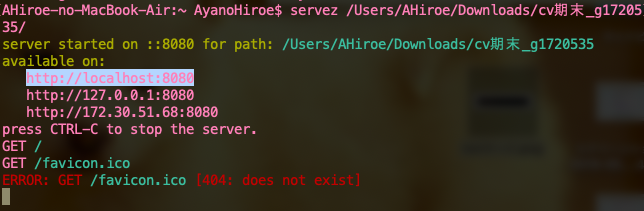
\includegraphics[width=150mm]{server.png}
 \caption{コマンド実行のスクリーンショット}
\end{center}
\end{figure}

\begin{figure}[h]
\begin{center}
 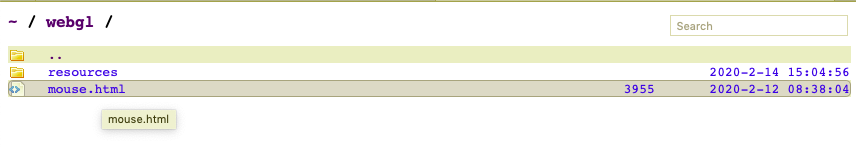
\includegraphics[width=150mm]{procedure.png}
 \caption{画面遷移のスクリーンショット}
\end{center}
\end{figure}

\begin{figure}[h]
\begin{center}
 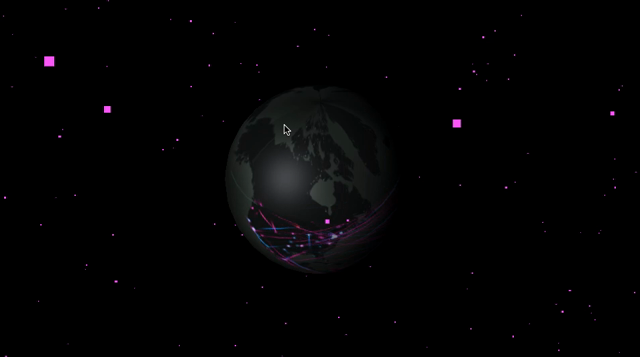
\includegraphics[width=150mm]{shot.png}
 \caption{実行結果のスクリーンショット}
\end{center}
\end{figure}
\end{document}
